%%%%
\tetePremStssBiom
\vspace*{-30pt}
\titreActivite{Hydrophilie, hydrophobie et micelle}

%%%% objectifs
\begin{objectifs}
  \item Comprendre la notion d'hydrophilie et d'hydrophobie.
  \item Voir la structure d'une micelle.
  \item Voir schématiquement la structure d'une membrane plasmique.
\end{objectifs}

\begin{contexte}
  Tous les êtres vivants sur Terre sont composés de une ou plusieurs cellules.
  Les cellules possèdent une membrane plasmique, qui permet de séparer l'intérieur, le cytoplasme, du milieu extérieur.
  
  \problematique{
    Quelles molécules permettent de former une membrane plasmique ?
  }
\end{contexte}


%%%% docs
\begin{doc}{Hydrophilie et hydrophobie}{doc:A_hydrophile_phobe}
  \begin{importants}
    Les molécules polaires sont dites \important{hydrophiles,} les molécules apolaires sont dites \important{hydrophobes.}
  \end{importants}
  Une molécule hydrophile («\textit{ qui aime l'eau} ») se mélangera bien dans l'eau, une molécule hydrophobe (« \textit{qui n'aime pas l'eau} ») ne se mélangera pas avec de l'eau.
\end{doc}

\begin{doc}{Molécules tensioactives}{doc:A_molecule_tensioactive}
  \begin{importants}
    Une molécule est dite \important{tensioactive} si elle possède une partie \important{hydrophobe} et une partie \important{hydrophile.}
  \end{importants}
  Les parties hydrophobes sont composées de carbones et d'hydrogènes (même électronégativité), tandis que les parties hydrophiles ont des azotes \azote, des oxygènes \oxygene\; et des phosphore \chemfig{P}.
  
  La plupart des lipides sont des tensioactifs.
  Les lipides sont composés d'une \important{tête hydrophile,} schématisé par un cercle, et d'une \important{queue hydrophobe,} schématisé par une vaguelette.
  
  \begin{center}
    \begin{tikzpicture}
      %% Choline
      \fill[color=yellow-400] (-6.9,-1.6) circle (0.7); 
      %% Glycérol
      \fill[color=purple-100] (-1.2, 0) -- (-1.2, -0.75) -- (0, -0.75) -- (0, -1.9)
        -- (-3.6, -1.9) -- (-3.6, -0.75) -- (-2.4, -0.75) -- (-2.4, 0);
      %% Phosphate
      \fill[color=orange-300] (-4,-1.6) circle (1.3);
      %% Acides gras
      \fill[color=cyan-200] (-0.7, -0.65) -- (5.1, -0.65) -- (5.1, 1.6) -- (3, 1.6)
        -- (3, 3) -- (0.7, 3) -- (0.7, 0.6) -- (-0.7, 0.6);
      \fill[color=cyan-200] (0.7,-0.85) -- (8, -0.85) -- (8, -2) -- (0.7, -2);
      %% Molécule
      \node at (0, 0) {\chemfig{!\phosphatidylcholine}};
    \end{tikzpicture}
  
    \legende{
      Phospholipide composé de deux \important[cyan-600]{acides gras} reliés à un groupe \important[orange-600]{phosphate} et un groupe \important[yellow-600]{choline} par un \important[purple-600]{glycérol}.
    }
  \end{center}
\end{doc}

\numeroQuestion
Entourer les deux groupes ester du phospholipide.

\question{
  Entourer le glycérol dans le phospholipide, puis donner sa formule brute.
}{
  La formule du glycérol est \chemfig{C_3 H_8 O_3}, c'est du propan-1,2,3-triol.
}[1]

\pasCorrection{\newpage \vspace*{-18pt}}
\begin{doc}{Micelles et couches-bilipidiques}{doc:A_micelle}
  \begin{wrapfigure}[12]{r}{0.33\linewidth}
    \centering
    \vspace*{-30pt}
    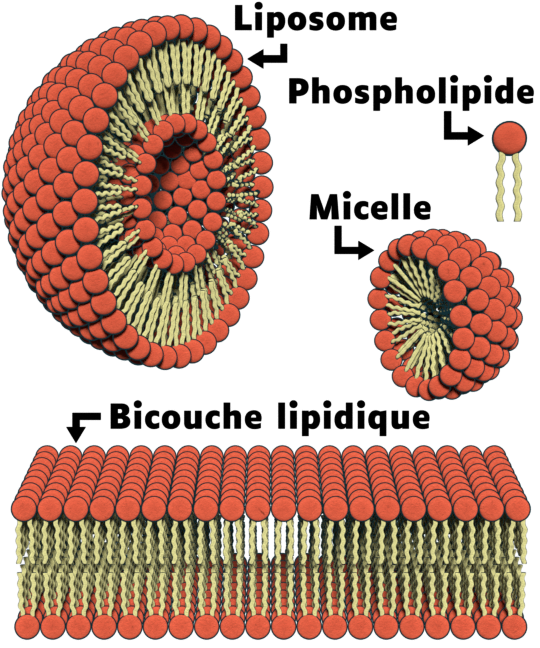
\includegraphics[width=0.95\linewidth]{images/molecules/biochimie/liposome_micelle_bicouche}
  \end{wrapfigure}

  La structure des molécules de lipides mène à la formation de structure particulière dans de l'eau liquide.
  Les queues hydrophobes étant repoussées par les molécules d'eau, elles vont s'agglomérer et former des structures ou les queues sont isolées de l'eau environnante : \important{les micelles,} avec un intérieur sans eau.
  \smallskip

  Si on a deux couches courbées composées de phospholipides, \important{une couche bi-lipidique,} on peut avoir la formation de \important{liposomes,} si la courbure est forte. Si la courbure est plus faible, on a formation de la base \important{d'une membrane cellulaire.}
  \smallskip
  
  Dans les \important{couches bi-lipidiques} les deux couches de lipides ont leurs têtes hydrophiles orientée vers l'extérieur, ce qui permet à leur queue hydrophobes de ne pas rentrer en contact avec de l'eau. 
  Ce sont les interactions électrostatiques entre les différentes parties de cette bicouche qui la pousse à former une sphère, avec un extérieur et un intérieur, comme une bulle de savon.
\end{doc}

\begin{doc}{Membrane cellulaire}{doc:membrane_cellulaire}
  \begin{wrapfigure}{r}{0.5\linewidth}
    \centering
    \vspace*{-36pt}
    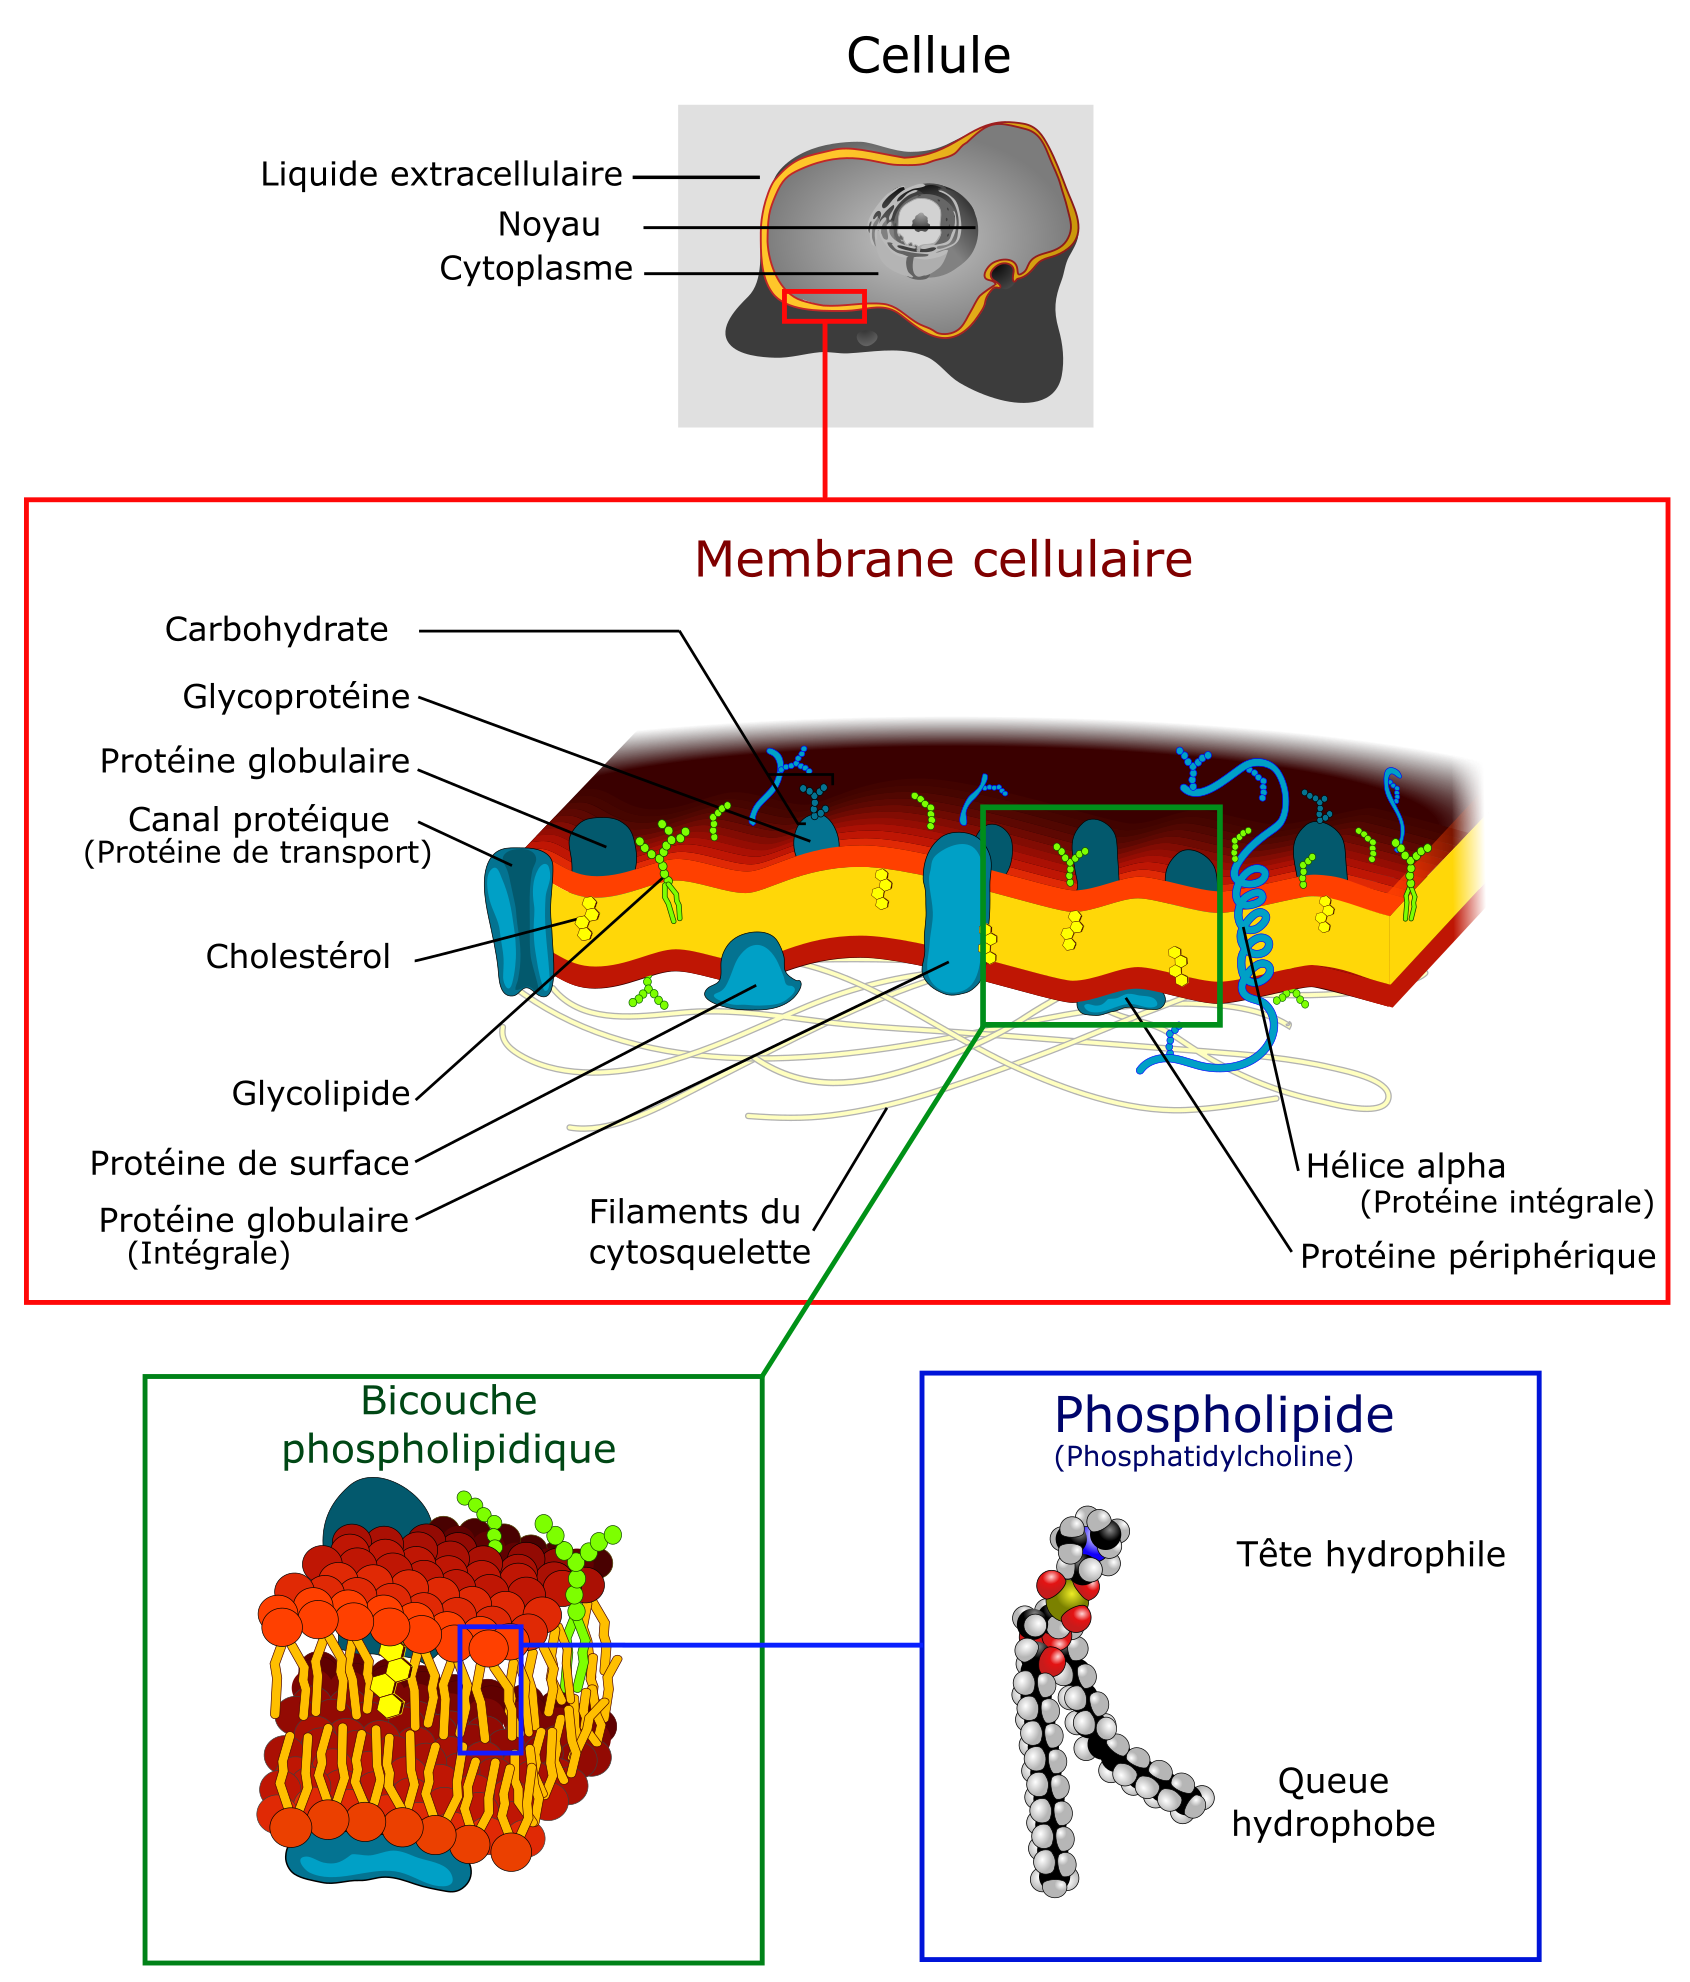
\includegraphics[width=1\linewidth]{images/molecules/biochimie/cellule_membrane_lipide.png}
  \end{wrapfigure}
  Les membranes cellulaires sont plus complexes qu'une simple couche bi-lipidique : elles sont aussi composées de \important{protéines,} qui permettent de renforcer la structure de la membrane cellulaire et de contrôler ce qui sort et ce qui entre de la cellule.
  \smallskip

  Les protéines sur la membrane plasmique font office de porte d'entrée pour la cellule. 
  Elles régulent la concentration de certains oligo-éléments dans la cellule, ou ne laissent entrer que les protéines qui ont la bonne géométrie.

  Comme les membranes se forment à partir de liaison électrostatique et non à l'aide de liaisons covalentes, elles sont très souples et peuvent prendre des formes très variées. 
  C'est le \important{cytosquelette} d'une cellule qui va déterminer sa forme, un peu comme les piquets d'une tente.
  
  \phantom{b}
\end{doc}

%%%%
\question{
  Recopier le phospholipide du document~\ref{doc:A_molecule_tensioactive}, et entourer sa partie hydrophobe et sa partie hydrophile.
}{
  La partie hydrophobe est composée des deux acides gras.
  La partie hydrophile est composée du groupe choline et du groupe phosphate.
}[5]
